 \section{Case Studies}
\label{sec:case_study}
To demonstrate the effectiveness of the Safety Annex, we describe two case studies.  



\iffalse
\subsection{Simple Wheel Brake System}
The Wheel Brake System (WBS) described in ARP4761 has been used as a case study for safety analysis, formal verification, and contract based design in numerous studies. In order to show scalability compare results with other tools and studies, the AADL model of the WBS used in~\cite{Stewart17:IMBSA} was enhanced using as a guide the NuSMV ARCH4 model as described in~\cite{DBLP:conf/cav/BozzanoCPJKPRT15}. This version of the WBS model was chosen due to the complexity of the model and because this model addresses required safety concerns (for description of these concerns, see~\cite{DBLP:conf/cav/BozzanoCPJKPRT15}). Due to the added complexity of this WBS system, a short description of the subcomponents and behavior is necessary. 

\subsubsection{Simple WBS architecture description}
The highest level model component is the WBS. It consists of the Braking System Control Unit (BSCU), green and blue hydraulic pressure lines (supplied by the green and blue hydraulic pumps respectively), a selector which selects between normal operating mode and alternate operating mode, and the wheel system. 

There are three operating modes of the WBS. In \textit{normal} mode, the system uses the \textit{green} hydraulic circuit. In \textit{alternate} mode, the system uses the \textit{blue} hydraulic circuit.  If the BSCU detects lack of pressure from the green line or one of its command units are invalid, then the system switches into alternate mode. The last mode of operation of the WBS is the \textit{emergency} mode. This is supported by the blue circut but operates if the blue hydraulic pump fails. The accumulator pump has a reserve of pressurized hydraulic fluid and will supply this to the blue circuit in emergency mode.  Antiskid braking commands receive data from the BSCU that will determine if skidding is found at the wheel and handle accordingly. 

In the simplified WBS model, there is one wheel that receives pressure from either the green or blue line. This wheel provides feedback to the BSCU providing information about the pressure supplied. 

To evaluate the effectiveness of the Safety Annex, we updated the simple WBS model~\cite{Stewart17:IMBSA} to specify faulty component behaviors. The components' nominal  and faulty behaviors are modeled separately. At the top-level AADL component, the fault hypothesis was specified as the maximum number of faults that can be active at any time. The AGREE contracts at the top-level component were verified using AGREE, with the ``Perform Safety Analysis'' option selected. This signals the tool to weave the nominal and faulty behaviors into one augmented AGREE model before feeding to the model checker.

In this example, the top level contract ``Pedal pressed and no skid implies brake pressure applied'' was verified in the presence of at most one fault active during execution.  However, it was shown to be invalid when more than one fault was allowed. The counterexample indicated that both Selector's outputs failed to non-deterministic values due to the faults introduced.
\fi


\subsection{Wheel Brake System}
The Wheel Brake System (WBS) described in ARP4761 has been used as a case study for safety analysis, formal verification, and contract based design in numerous studies. In order to show scalability compare results with other tools and studies, the AADL model of the WBS used in~\cite{Stewart17:IMBSA} was enhanced using as a guide the NuSMV ARCH4 model as described in~\cite{DBLP:conf/cav/BozzanoCPJKPRT15}. This version of the WBS model was chosen due to the complexity of the model and because this model addresses required safety concerns (for description of these concerns, see~\cite{DBLP:conf/cav/BozzanoCPJKPRT15}). Due to the added complexity of this WBS system, we provide a short description of the subcomponents and behavior. 

\subsubsection{WBS architecture description} 
The WBS is composed of two main systems: the control system and the physical system. The control system electronically controls the physical system and contains a redundant Braking System Control Unit (BSCU) in case of failure. The physical system consists of the hydraulic circuits running from hydraulic pumps to wheel brakes. This is what provides braking force to each of the 8 wheels of the aircraft. 

Just as in the simple WBS model, there are three operating modes. In \textit{normal} mode, the system uses the \textit{green} hydraulic circuit. The normal system is composed of the green hydraulic pump and one meter valve per each of the 8 wheels. Each of the 8 meter valves are controlled through electronic commands coming from the BSCU. These signals provide brake commands as well as antiskid commands for each of the wheels. The braking command is determined through a sensor on the pilot pedal position. the antiskid command is calculated based on information regarding ground speed, wheel rolling status, and braking commands. 

In \textit{alternate} mode, the system uses the \textit{blue} hydraulic circuit.  The wheels are all mechanically braked in pairs (one pair per landing gear). The alternate system is composed of the blue hydraulic pump, four meter valves, and four antiskid shutoff valves. The meter valves are mechanically commanded through the pilot pedal corresponding to each landing gear. If the system detects lack of pressure in the green circuit, the selector valve switches to the blue circuit. This can occur if there is a lack of pressure from the green hydraulic pump, if the green hydraulic pump circuit fails, or if pressure is cut off by a shutoff valve. If the BSCU unit becomes invalid, the shutoff valve is closed. 

The last mode of operation of the WBS is the \textit{emergency} mode. This is supported by the blue circut but operates if the blue hydraulic pump fails. The accumulator pump has a reserve of pressurized hydraulic fluid and will supply this to the blue circuit in emergency mode. 

\subsubsection{Fault Analysis of WBS using Safety Annex}
After the verification was completed, we defined faults equivalent to those described in the xSAP model for the NuSMV WBS system in~\cite{DBLP:conf/cav/BozzanoCPJKPRT15}. A description of modelling metrics can be found in Figure~\ref{fig:metrics}.

\begin{figure}[h!]
	\vspace{-0.17in}
	\begin{center}
		%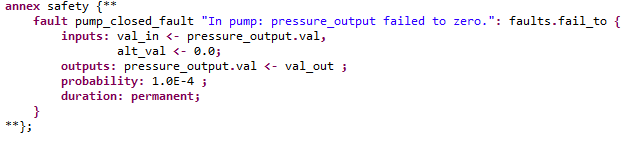
\includegraphics[trim=0 330 150 0,clip,width=1.0\textwidth]{images/pump_fault.png}
		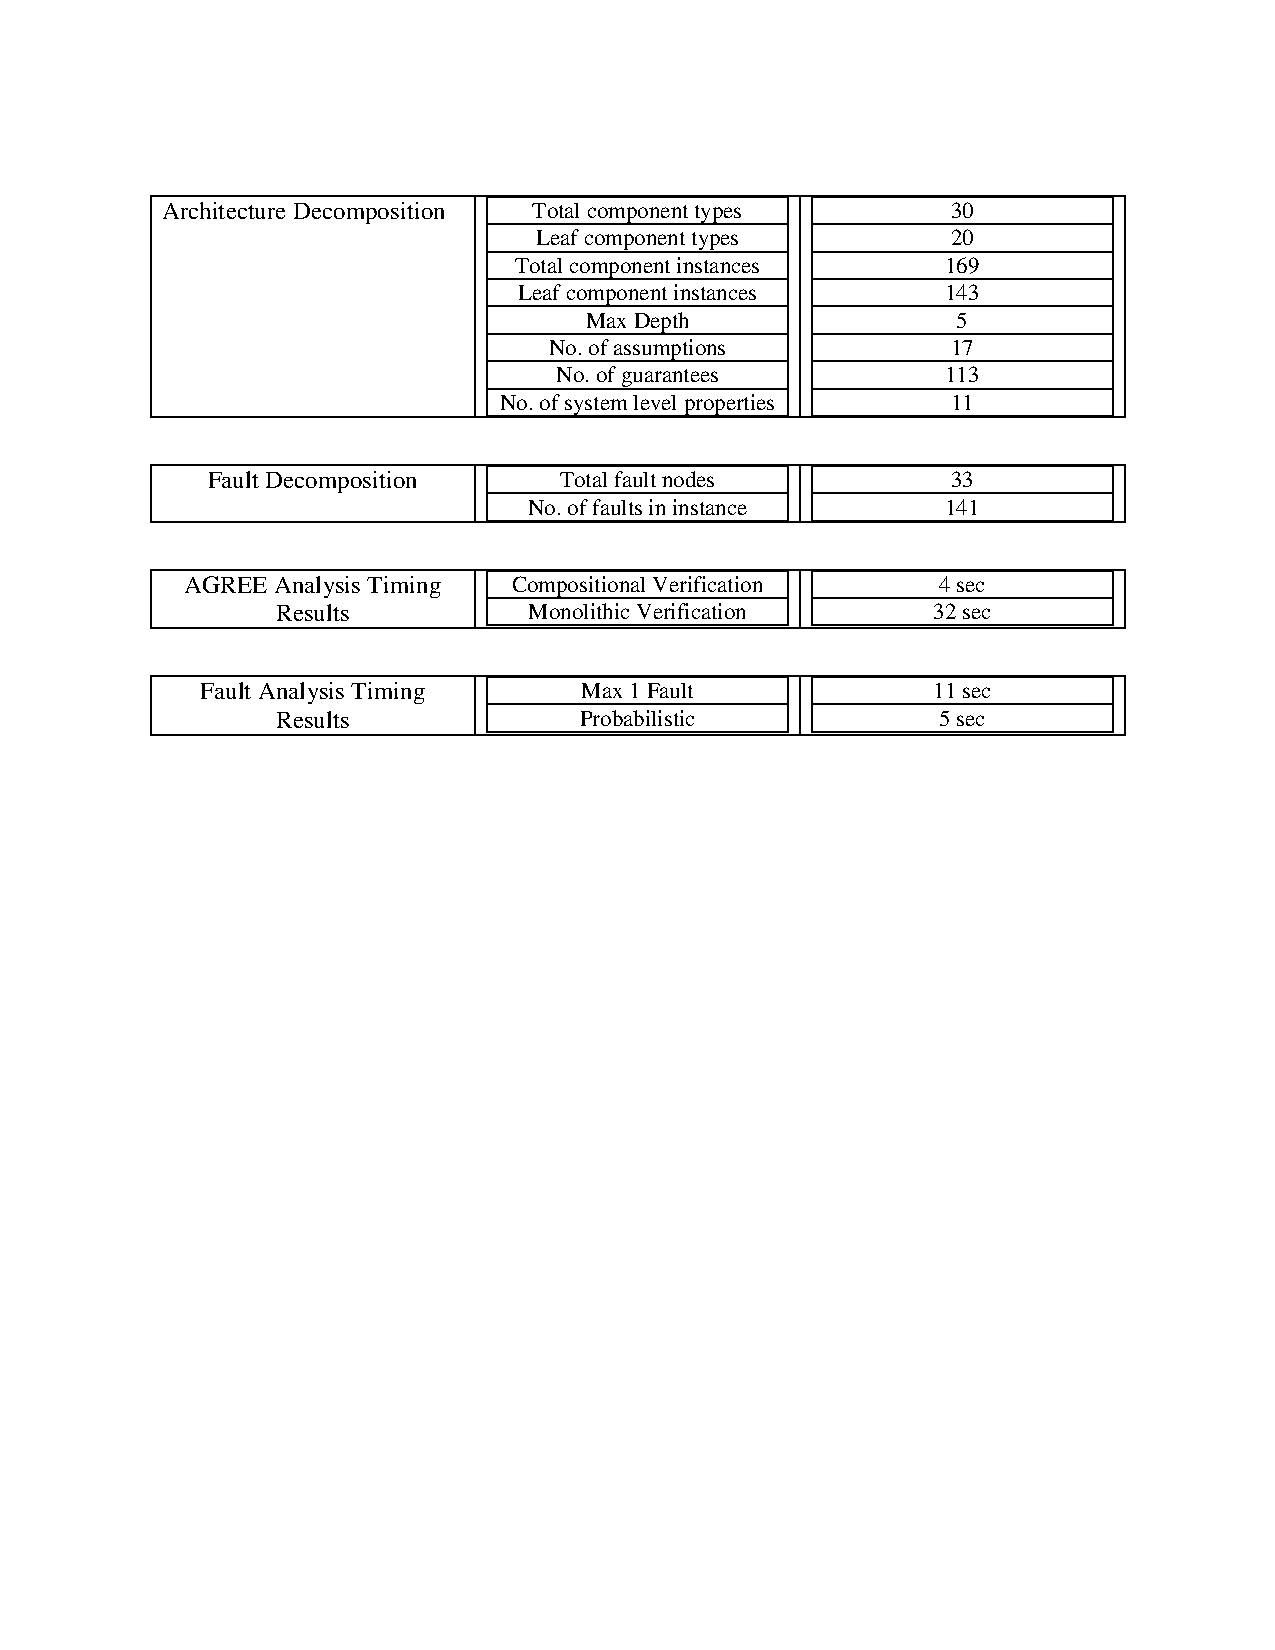
\includegraphics[trim=0 435 0 90,clip,width=1.0\textwidth]{images/arch_table.pdf}
		\caption{Modeling, Verification, and Fault Analysis Metrics}
 		\label{fig:metrics}
	\end{center}
	\vspace{-0.40in}
\end{figure}

Fault analysis on the top level WBS system was performed using two metrics: maximum one fault and probabilistic. Of the eleven top level properties, the ones that did not pass either analysis were regarding the safety requirement: \textit{Inadvertant braking at the wheel}. This was caused by a fault on the pedal position sensor. This sensor determines if the mechanical brakes are pressed. If so, it sends an electrical command to the BSCU to command braking. The fault was an inverted boolean fault which inverted the mechanical pedal value (false) and created a true electrical pedal value. Thus, we have a situation where no  braking is commanded mechanically, but braking is commanded electronically nonetheless. 

The system design decisions regarding pedal position sensors are based on the NuSMV model. Using this system implementation, it is not resilient to a single fault. The analysis provides a clear counterexample to the invalid top level properties. In terms of the safety analysis process, this corresponds with the SSA results feeding back into the FTA. Discussion is required to determine if the likelihood of this sensor fault is sufficiently low given the exposure time frame window or if sensor redundancy must be applied in order to increase reliability. This information can then be used during the next phase of system development. 


\subsection{Quad-Redundant Flight Control System}
In order to discuss Byzantine faults and hardware errors with their propogations, we applied the Safety Annex to the Quad-Redundant Flight Control System (QFCS) model~\cite{QFCS15:backes}. Faulty behaviors were introduced in order to see the response of the system to several faults, and to evaluate fault mitigation logic in the model.  The QFCS system-level properties failed when unhandled faulty behaviors were introduced.

We also used the Safety Annex to explore more complicated faults at the system level on a simplified QFCS model with cross-channel communication between its Flight Control Computers.

\begin{itemize} 
	\item Byzantine faults~\cite{Driscoll-Byzantine-Fault} were simulated by creating one-to-one connections from the source to multiple observers so that disagreements could be introduced by injecting faults on individual outputs. A system-level property failed due to the fault on the baseline model, but did not fail on the model with Byzantine fault handling protocol added. Using the Safety Annex like this can test a system's vulnerability to Byzantine faults and verify mitigation mechanisms.
	
	\item Dependent failures in hardware were modeled by injecting faults to hardware components (physical layer), and faults to software components (logical layer) that are bound to the hardware components, then specifying fault propagations at the QFCS system level to indicate that the software faults are dependent on the hardware faults.
\end{itemize}


